\documentclass{cheatsheet}
\usepackage{bm}
\usepackage{textcomp, mathcomp}
\usepackage{empheq}
\usepackage{pbox}
\usepackage{booktabs}
\usepackage{verbatim}
\usepackage{graphicx}
\usepackage{tabu}

\doctitle{Control Systems I Cheatsheet}
\author{Christian Leser \\ \vspace*{-0.2em}}

\begin{document}
\section{1. Terminology}
	\subsection{1.1 Input, Output, State}
    %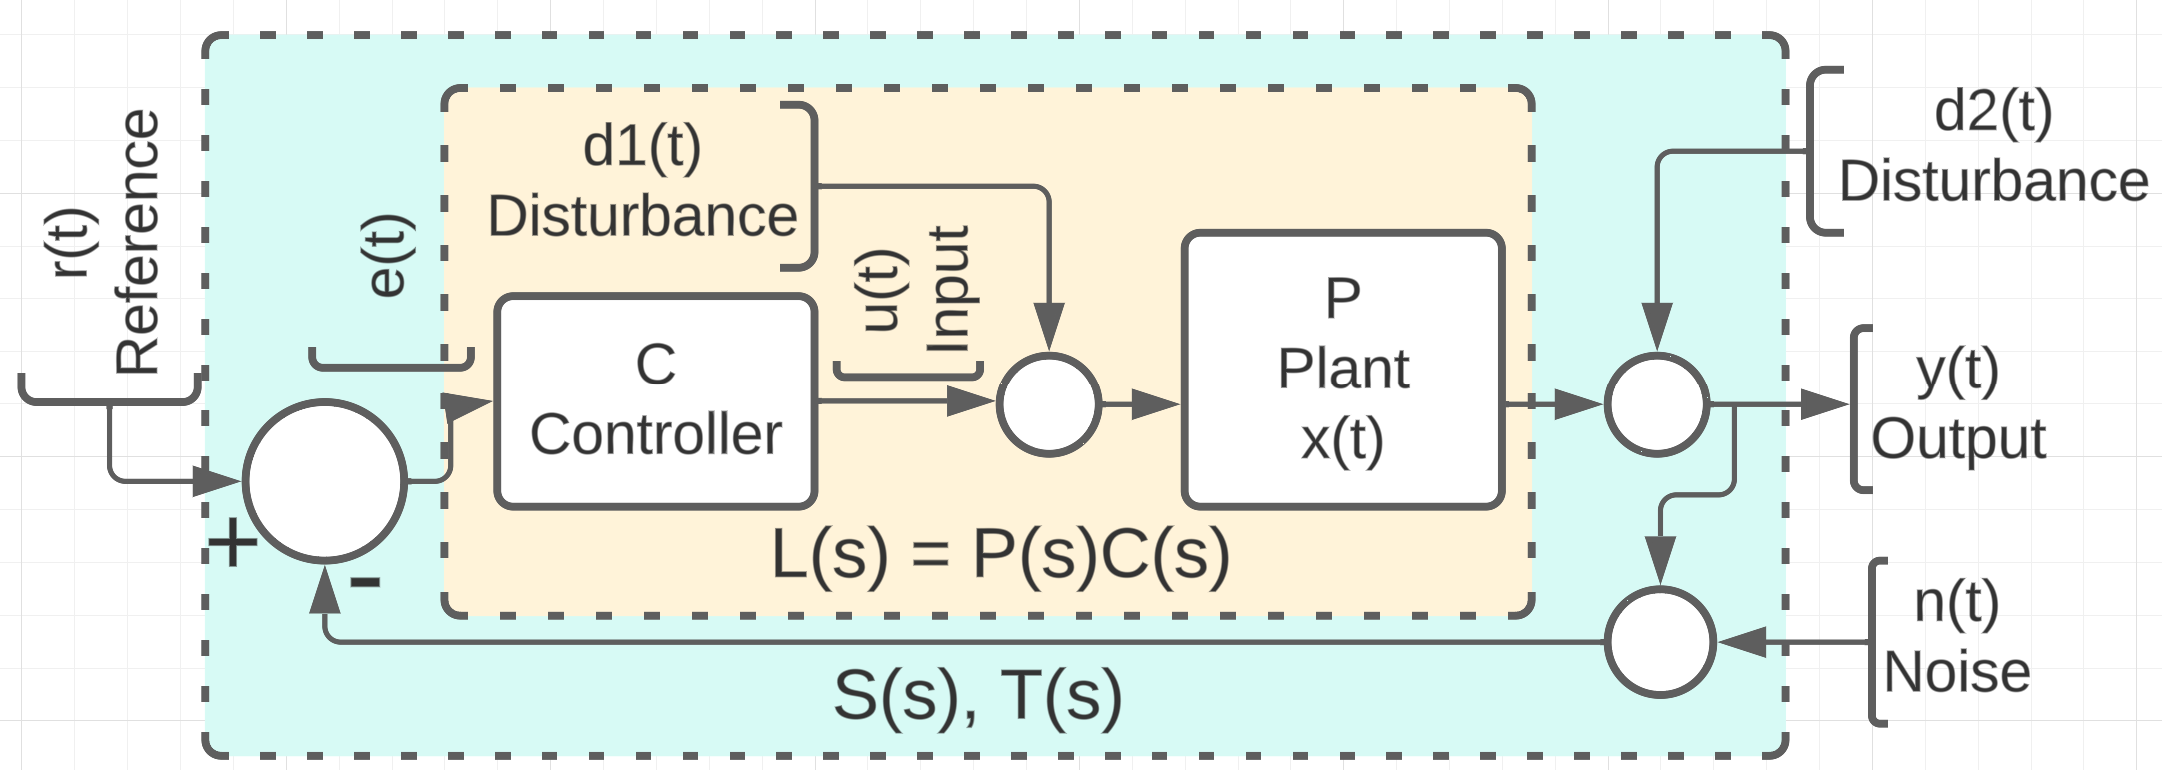
\includegraphics[width = \linewidth]{src/images/basic_block_chart.png}
    \begin{itemize}
        \item \textbf{(Control) Input u(t)} (gas pedal)
        \begin{itemize}
            \item endogenous: manipulation by designer
            \item exogenous: generated by environment (e.g. Weather)
        \end{itemize}
        \item \textbf{Output / Measurement y(t)} (speed)
        \begin{itemize}
            \item measured outputs: Quantities that we can measure
            \item performance outputs: unmeasurable but controllable (e.g. average fuel consumption)
        \end{itemize}
        \item \textbf{state x(t)}: "memory", summary of all past inputs (fuel)
        \item parameter: quantities that do not change over time (colour)
\end{itemize}
	\subsection{Classification}
    \textcolor{blue}{L}\textcolor{orange}{TI} \textcolor{teal}{SISO}: \textcolor{blue}{Linear} \textcolor{orange}{Time invariant} \textcolor{teal}{single input single output}
    \subsubsection*{Linear vs. nonlinear Systems}
        For a linear system, Additivity and Homogenity must hold:
        \begin{align*}
            \Sigma (\alpha u_a + \beta u_b) = \alpha (\Sigma u_a) + \beta (\Sigma u_b) = \alpha y_a + \beta y_b
        \end{align*}
        Therefore, superposition holds for linear systems.\\
        Linear System can be represented in state-space-form, the matrices do not depend on time:
        \begin{equation}\label{eqn:LTI}
            \begin{cases}
                \dot{x}(t) = Ax(t) + Bu(t)\\
                y(t) = Cx(t) + Du(t)
            \end{cases}
        \end{equation}

    \subsubsection*{Causal vs non-causal systems}
        Output at time $t$ depends only on the values of input on $(-\infty, t]$ (future inputs do not affect current output)\\
        $y(t) = f(u(\tau)), \tau < t$
    
    \subsubsection*{Static systems}
        Static (memoryless) vs Dynamic
        y(t) only depends on u(t), output does not depend on past or future\\
        $dim(x) = 0$ : dimension of system equals 0

    \subsubsection*{Time invariant vs Time-varying !überarbeiten!}
        output does not depend on time, only on $\Delta t$ (counter example sun clock)\\
        {\centering\textbf{\underline{Time-varying}}}
        \begin{equation}
            t_0 = t_0
            \begin{cases}
                \dot{x}(t) = f(t, x(t), u(t))\\
                y(t) = g(t, x(t), u(t))
            \end{cases}
            \rightarrow
            \begin{cases}
                \dot{x}(t) = A(t)x(t) + B(t)u(t)\\
                y(t) = C(t)x(t) + D(t)u(t)
            \end{cases}
        \end{equation}

        {\centering\textbf{\underline{Time Invariant}}}
        \begin{align*}
            \text{time shift operator $\sigma_{\tau}$:\quad \quad} \sigma_{\tau} y(t) = \Sigma \sigma_{\tau} u(t)\\
            y(t - \tau) = \Sigma(u(t - \tau))\\
            t_0 = 0
            \begin{cases}
                \dot{x}(t) = f(x(t), u(t))\\
                y(t) = g(x(t), u(t))
            \end{cases}
            \rightarrow
            \begin{cases}
                \dot{x}(t) = Ax(t) + Bu(t)\\
                y(t) = Cx(t) + Du(t)
            \end{cases}
        \end{align*}
	\subsection{Interconnections}
    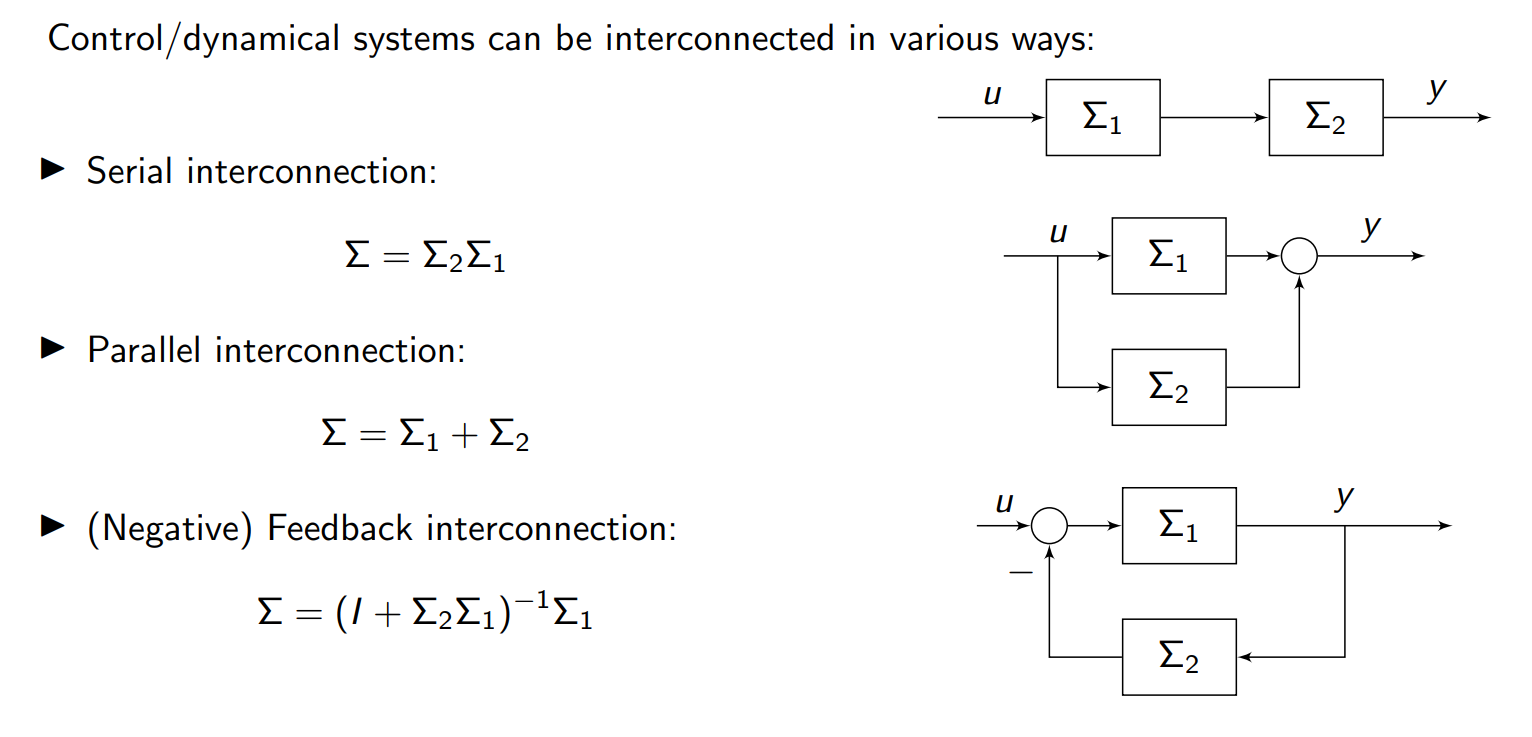
\includegraphics[width = \linewidth]{src/images/interconnection.png}
%	\subsection{Basic Control Architectures}
    \begin{tabu}{X[m] X[2, c, m]}
        \textbf{Name}               & \textbf{Block chart}\\
        \hline \hline
        Feed-forward      & 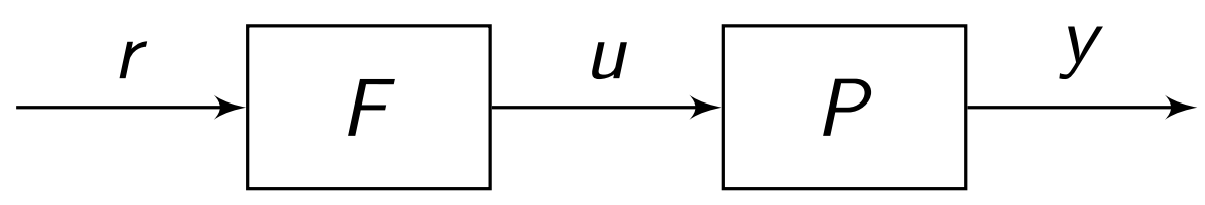
\includegraphics[width = \linewidth]{src/images/architecture_feed_forward.png}\\
        \hline
        Feedback    & 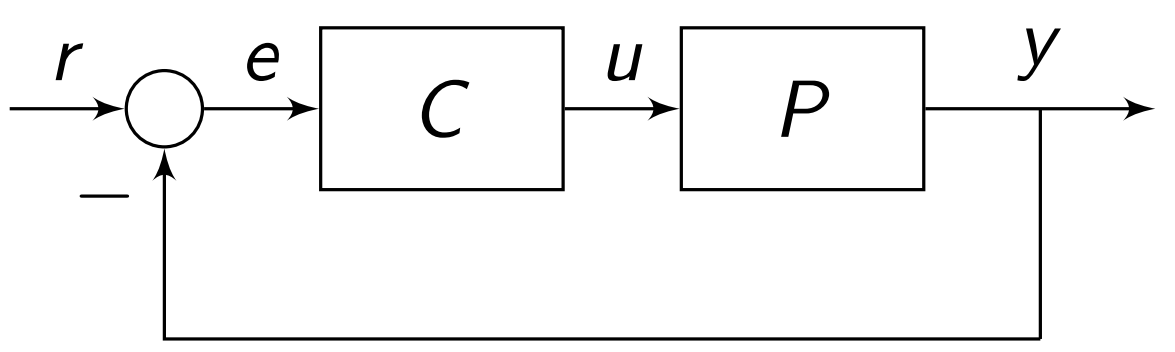
\includegraphics[width = \linewidth]{src/images/architecture_feedback.png}\\
        \hline
        Two degrees of freedom    & 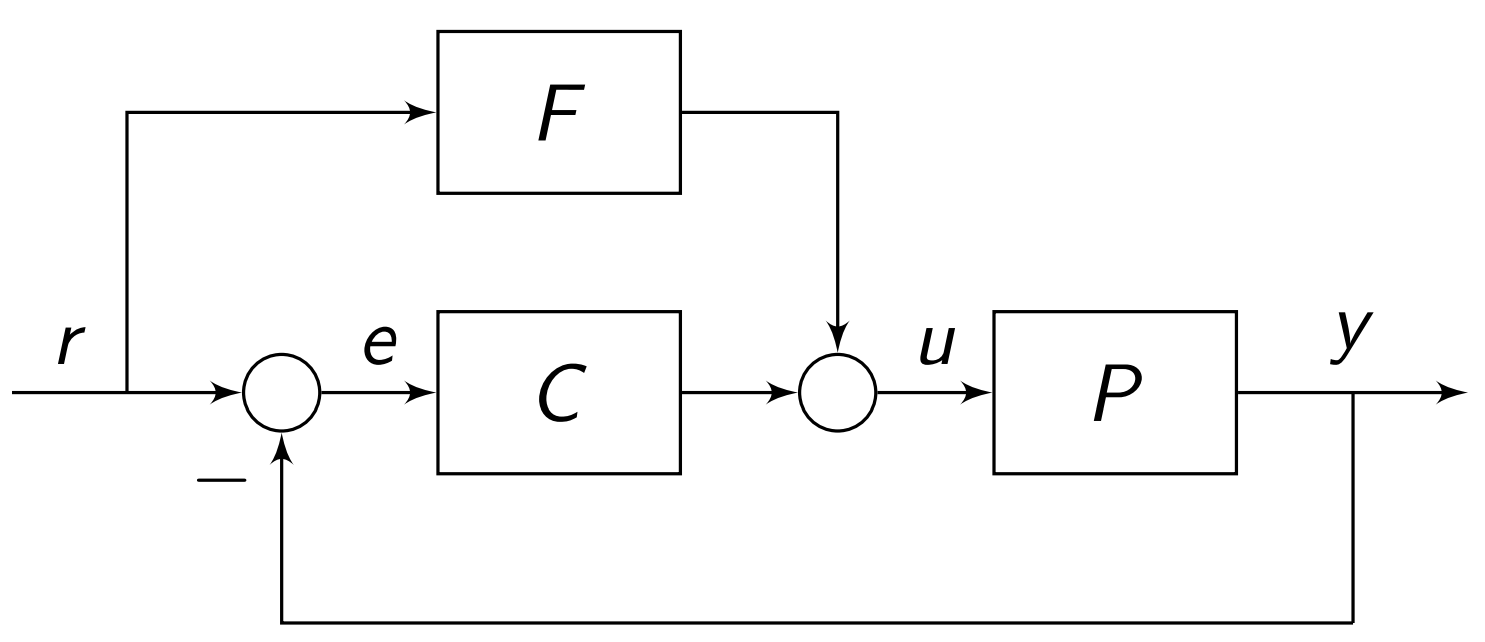
\includegraphics[width = \linewidth]{src/images/architecture_two_freedom.png}
    \end{tabu}

\section{2. System Modeling}
	for LTI SISO systems: $\frac{d}{dt} \text{storage} = \sum \text{inflows} - \sum \text{outflows}$

    \begin{center}
        \textbf{\underline{Mass conservation}}    
    \end{center}
    \begin{align*}
        \frac{d}{dt} m = \sum m_{in}(t) - \sum m_{out}(t)
    \end{align*}

    \begin{center}
        \textbf{\underline{Mechanical systems}}    
    \end{center}
    \begin{align*}
        M(t) = J \cdot \ddot{\phi}(t)
    \end{align*}

    \begin{center}
        \textbf{\underline{Thermodynamic systems}}    
    \end{center}
    \begin{align*}
        m \frac{d}{dt} T(t) = c(T_{ext}(t) -T(t)) + u(t)
    \end{align*}
	\subsection{State Space Form}
    \begin{minipage}{0.49 \linewidth}
        \begin{center}
            \textbf{\underline{General form}}
        \end{center}
        \begin{align*}
            \begin{cases}
                \dot{x}(t) = f(x(t), u(t), d(t))\\
                y(t) = f(x(t), u(t), d(t))
            \end{cases}
        \end{align*}
    \end{minipage}
    \begin{minipage}{0.49 \linewidth}
        \begin{center}
            \textbf{\underline{Linear System}}
        \end{center}
        \begin{align*}
            \begin{cases}
                \dot{x}(t) = Ax(t) + Bu(t)\\
                y(t) = Cx(t) + Du(t)
            \end{cases}\\
        \end{align*}
    \end{minipage}
    dim$(x) = $ Order/Dimension (min. $\#$ of variables to describe state)
    
	\subsection*{Jacobian Linearization Process}
    Use in LTI-Systems\\
    Equilibrium point (state does not change): $\dot{x} = f(x_e, u_e) = 0$\\
    Linearized systems are accurate around equilibrium:
    \begin{align*}
        \left(
            \begin{array}{c}
                x\\
                u
            \end{array}
        \right)
        \approx
        \left(
            \begin{array}{c}
                x_e\\
                u_e
            \end{array}
        \right)
    \end{align*}
    \begin{align*} % \Big\rvert_{x = x_e, u = u_e} Auswertung der Differentiale
        A &= 
        \left[\begin{array}{c c c}
            \frac{\partial f_1}{\partial x_1} & \cdots & \frac{\partial f_1}{\partial x_n}\\
            \vdots & \ddots & \vdots\\
            \frac{\partial f_n}{\partial x_1} & \cdots & \frac{\partial f_n}{\partial x_n}
        \end{array}\right]
        &B &= 
        \left[\begin{array}{c}
            \frac{\partial f_1}{\partial u}\\
            \vdots\\
            \frac{\partial f_n}{\partial u}
        \end{array}\right]
        \\
        C &= 
        \left[\begin{array}{c c c}
            \frac{\partial g}{\partial x_1} & \cdots & \frac{\partial g}{\partial x_n}
        \end{array}\right]
        &D &= 
        \left[\begin{array}{c}
            \frac{\partial g}{\partial u}
        \end{array}\right]
    \end{align*}
	\subsection{time response to LTI system}
    \begin{center}
        \textbf{Superposition of responses:}
    \end{center}
    
    \begin{minipage}{0.49\linewidth}
        \begin{minipage}{0.49\linewidth}
            non-zero initial conditions (natural response)
        \end{minipage}
        \begin{minipage}{0.49\linewidth}
            \begin{align*}
                \begin{cases}
                    x(0) = x_0\\
                    u(t) = 0
                \end{cases}
            \end{align*}
        \end{minipage}
    \end{minipage}
    \begin{minipage}{0.49\linewidth}
        \begin{minipage}{0.44\linewidth}
            non-zero inputs (forced response)
        \end{minipage}
        \begin{minipage}{0.54\linewidth}
            \begin{align*}
                \begin{cases}
                    x(0) = 0\\
                    u(t) = u(t)
                \end{cases}
            \end{align*}
        \end{minipage}
    \end{minipage}
    \begin{align*}
        x(t) &= \underbrace{e^{At} \cdot x_0}_{\substack{\text{hom. solution}\\ u(t) = 0}} + \underbrace{\int\limits_0^t e^{A (t-\rho)} B u(\rho) d\rho}_{\substack{\text{inhom. solution, zero initial condition}\\ x(0) = 0}}\\
        y(t) &= \underbrace{C \cdot e^{At} \cdot x_0}_{\substack{\text{natural / initial} \\ \text{condition response}}} + \underbrace{C \cdot \int\limits_0^t e^{A (t-\rho)} B u(\rho) d\rho}_{\text{forced response}} + \underbrace{D u(t)}_{\text{feedthrough}}
    \end{align*}

    state transition function: $\psi(t) = e^{At}$ %Maybe how to get the solution of an lti? see lecture 4 Time response
	\subsection{Stability}
    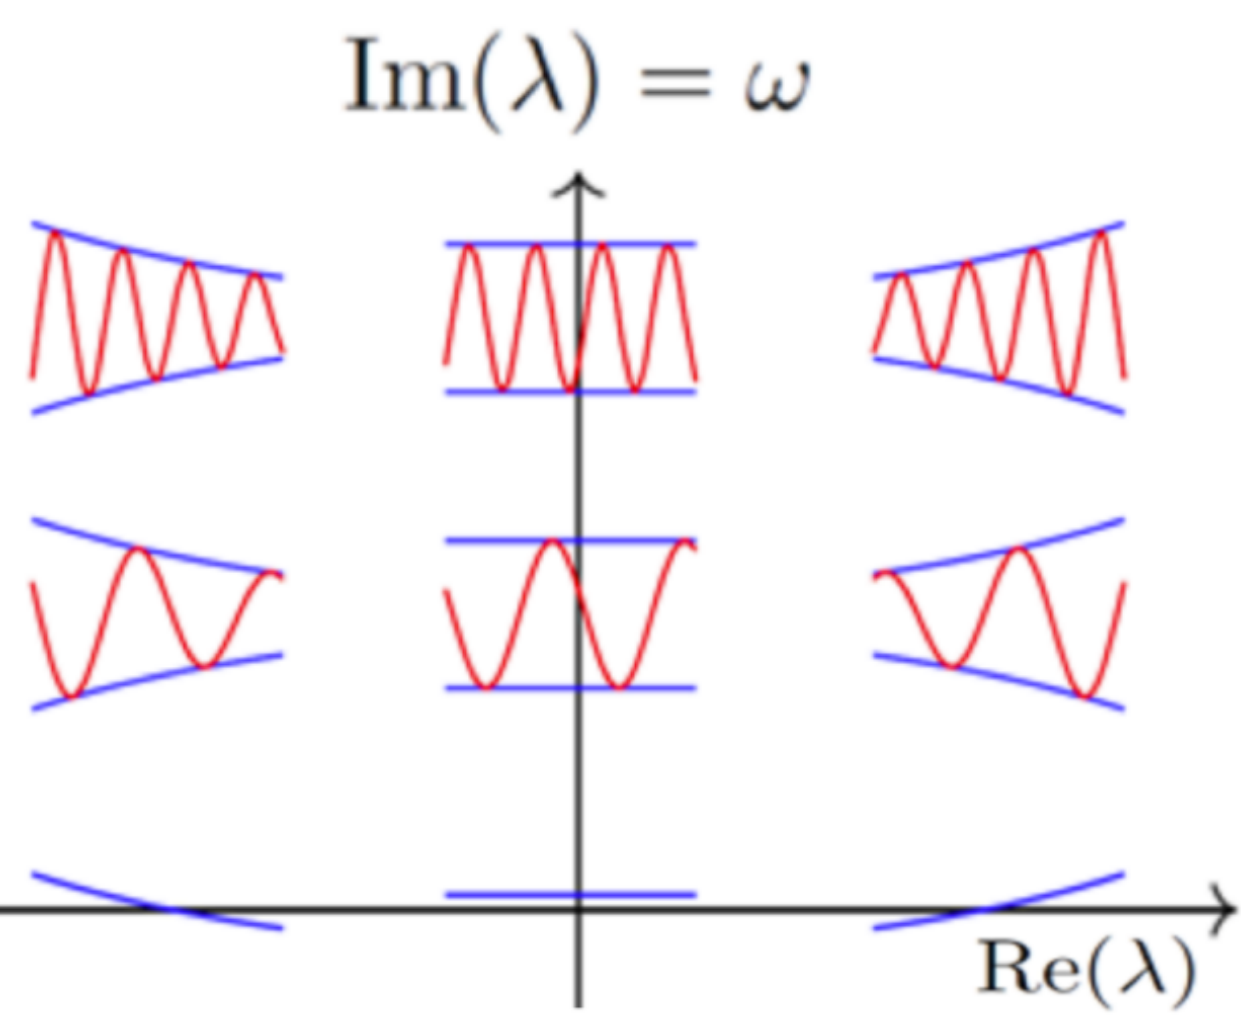
\includegraphics[width = \linewidth]{src/images/eigenvalue_response.png}
    system behaviour based on eigenvalues of A

    \subsubsection{Lyapunov stable}
    $\lim_{t \rightarrow \infty} x(t) \neq \pm \infty \Leftrightarrow Re(\lambda_i) \leq 0 \text{, exactly one } Re(\lambda_i) = 0$

    \subsubsection{Asymptotically stable}
    $\lim_{t \rightarrow \infty} x(t) = 0 \Leftrightarrow Re(\lambda_i) < 0$

    \subsubsection{BIBO (Bounded Input Bounded Output) stability}
    $\lim_{t \rightarrow \infty} y(t) \neq \pm \infty \Leftrightarrow Re(\lambda_i) < 0$

    \begin{center}
        \textbf{Not stabilizable and observable systems}
    \end{center}
    \begin{tabu}{|X[6] X X[3]|}
        \hline
        asymptotically stable & $\rightarrow$ & BIBO stable\\
        ? & $\leftarrow$ & BIBO stable\\
        Lyap. stable or unstable & $\rightarrow$ & ?\\
        Lyap. stable or unstable & $\leftarrow$ & BIBO unstable\\
        \hline
    \end{tabu}

    \subsubsection{Unstable}
    $\lim_{t \rightarrow \infty} x(t) = \pm \infty \Leftrightarrow Re(\lambda_i) > 0 \text{for at least one i}$

\section{System Analysis}

\section{System Synthesis}

\section{Appendix}
	\subsection{compute matrix exponential}
    \subsubsection{Taylor expansion}
        \begin{align*}
            e^{At} = I + At + \frac{1}{2}(At)^2 + ... + \frac{1}{n!}(At)^n + ...
        \end{align*}
    \subsubsection{Diagonalization}
        \begin{align*}
            A &= TDT^{-1}\\
            \Rightarrow exp(At) &= T e^{Dt} T^{-1}\\
            &= T \text{diag}(e^{\lambda_1 t}, e^{\lambda_2 t}, ..., e^{\lambda_n t}) T^{-1}\\
            T &= (EV_1, EV_2, ..., EV_n)
        \end{align*}
    \subsubsection{Jordan matrix}
        \begin{align*}
            exp\left(
                \left[
                    \begin{array}{c c c}
                        \lambda & 1 & 0\\
                        0 & \lambda & 1\\
                        0 & 0 & \lambda
                    \end{array}
                \right]
                t
            \right)
            =
            \left[
                \begin{array}{c c c}
                    1 & t & \frac{1}{2!} t^2\\
                    0 & 1 & t\\
                    0 & 0 & 1
                \end{array}
            \right]
            e^{\lambda t}
        \end{align*}
	\subsection{Euler Formula}
    \begin{align*}
        &e^{js} = cos(js) + j sin(js)\\
        &cos(s) = \frac{e^{js} + e^{-js}}{2} \quad \quad sin(s) = \frac{e^{js} - e^{-js}}{2j}
    \end{align*}

\end{document}

\begin{comment}
	TERMINOLOGY
	Definitions from ZF
Input, output, state…
	Classification of Systems (Also see ZF)
SYSTEM MODELING / transfer real world problems to input output system
	Thermodynamics
	Conservation of mass: for LTI SISO systems: $\frac{d}{dt} \text{storage} = \sum \text{inflows} - \sum \text{outflows}$

	Mechanics
NETWORK ANALYSIS
	(Interconnections & Basic Control Architectures) (Block Diagrams on ZF)
LINEARIZATION
	Jacobian Linearization process
LINEAR SYSTEM ANALYSIS
TIME RESPONSE
STABILITY
	Equilibrium point: $\dot{x}(t) = 0
FREQUENCY DOMAIN
	y(t) = G(s) * u(t) for u(t) = e^(st)
	Therefore, for sinusoidal inputs: u(t) = cos(omega * t) -> y = M cos(omega * t + phi), M = |G(j * omega)|, phi = \angle G(j * omega
	e^(i*s*t) = cos(s*t) + i*sin(s*t), cos(s*t) = 
	STATE SPACE -> TRANSFER FUNCTION
	TRANSFER FUNCTION -> CONTROLLABLE CANONICAL FORM
	POLES/ZEROS
SIMPLE LAPLACE
	derivative of a laplace function
	laplace of step function
	laplace of x^n

	!!! Disturbance and Noise rejection !!!
\end{comment}